\chapter{Implementation}
\label{ch:implementation}
This chapter presents the technical implementation of the dynamic and heterogeneous crowd computing platform in detail. The implementation leverages modern web technologies introduced in chapter \ref{ch:methodology} to create a high-performance distributed computing solution for the web. At its core, the system utilizes WebAssembly for cross-platform compatibility, high performance, and language independence (\ref{sec:methodology:wasm}), WebSockets for efficient bidirectional communication (\ref{sec:methodology:websokets}), and WebWorkers for potential parallel Task execution (\ref{sec:methodology:webworker}).

The following sections describe the components of the architecture, communication sequences, scheduling strategies, persistence mechanisms and the challenges encountered during the implementation phase. Sections \ref{sec:implementation:backend} and \ref{sec:implementation:frontend} describe the interaction with the platforms API and web interface.

\section{Architecture}
\label{sec:implementation:architecture}
The platform consists of the following three components:
\begin{itemize}
    \item Backend (Server) as the central component handling the distribution of Tasks and persistence of Job results \ref{sec:implementation:backend}, implemented using Nest.js \cite{methodology:nestjs}
    \item Frontend providing the web application for all Clients \ref{sec:implementation:frontend}, implemented using Next.js \cite{methodology:nextjs}
    \item Database for persisting Job and User data, implemented with PostgreSQL \cite{methodology:db}
\end{itemize}

Figure \ref{fig:implementation:architecture} illustrates the architecture of the platform. Heterogenous clients, diverse in hardware and operating system, are able to connect to the platform. Clients access the platform throuh the Frontend which than establish the WebSocket communication to the Server using the Socket.IO library. Each client (Worker and Administrator) maintains a bidirectional WebSocket connection to the Server. The database is exclusively accessible by the Server.

\begin{figure}[htbp]
    \centering
    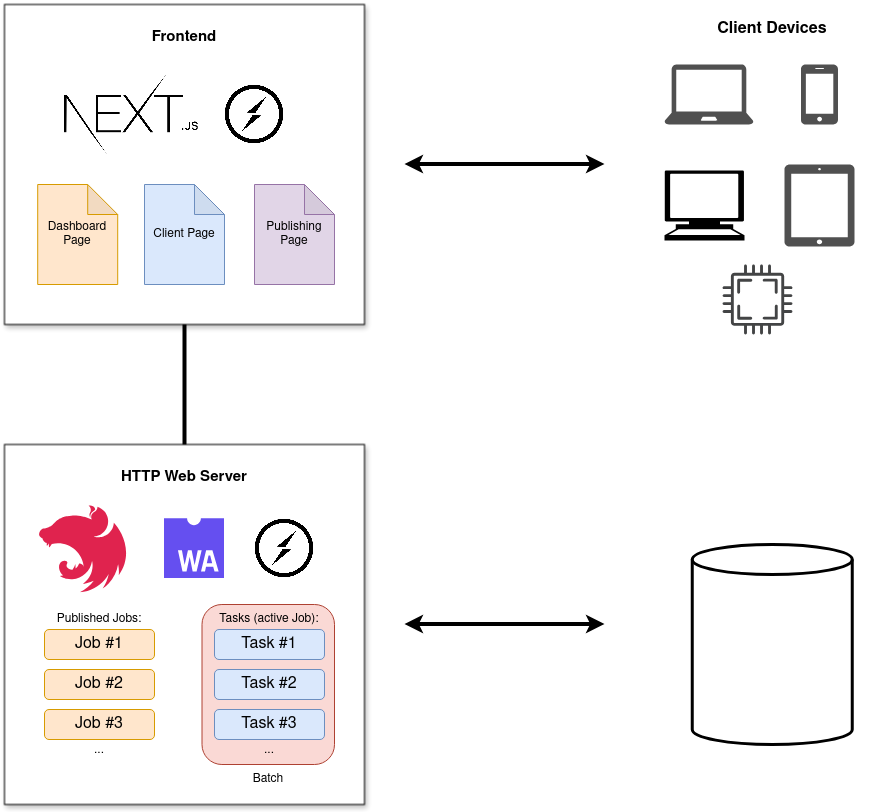
\includegraphics[width=0.95\textwidth]{gfx/figures/WebAssembly-MA.png}
    \caption{Architecture (Draft)}
    \label{fig:implementation:architecture}
\end{figure}

\subsection{Communication}
\label{subsec:implementation:architecture:communication}
When clients establish a connection to the platform by accessing the frontend application, a WebSocket connection is initiated. This enables real-time and bidirectional communication between the Server and client. Therefore this connection is used to send Tasks from the Server to the Workers as well to send the result of each Tasks from the Workers back to the Server. Furthermore, Administrators receive real-time data about all connected Workers and the current status of each Job through this WebSocket connection.

\begin{figure}[htbp]
    \centering
    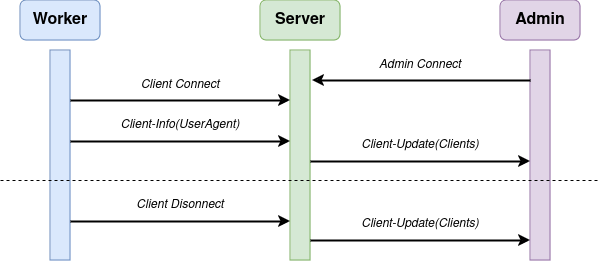
\includegraphics[width=0.95\textwidth]{gfx/figures/communication-connection.png}
    \caption{Communication: Connection of Worker \& real-time Update for Administrator}
    \label{fig:implementation:communication1}
\end{figure}

Figure \ref{fig:implementation:communication1} illustrates the process of a Worker connecting to the Server. Upon successful connection, the Worker transmits all available information regarding its hardware and operating system in form of the Browser User Agent to the Server. After this initialization of the Worker, all previously connected Administrators automatically receive an updated list of all connected Workers. Similarly, if a Worker disconnects a automatic update is send to all Administrators.

\begin{figure}[htbp]
    \centering
    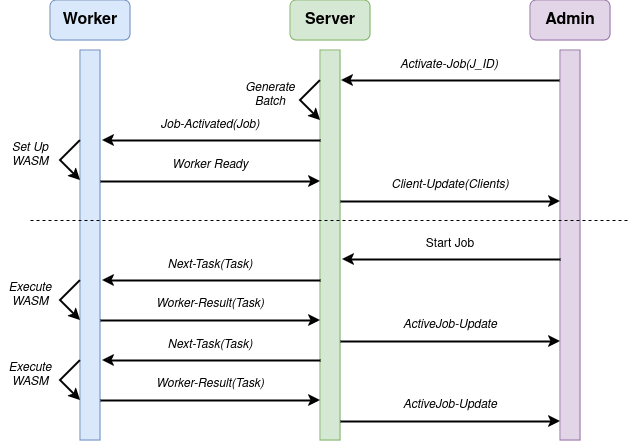
\includegraphics[width=0.95\textwidth]{gfx/figures/communication-jobexecution.png}
    \caption{Communication: Administrator starts Job \& Worker execute Tasks}
    \label{fig:implementation:communication2}
\end{figure}

Figure \ref{fig:implementation:communication2} illustrates the Job initiation and execution process. The sequence begins when an Administrator changes a Jobs status to \emph{ACTIVE}. The Server then generates a Batch of Tasks for the specified Job and notifies all connected Workers by transmitting the activated Job to them. Upon receiving this notification, each Worker retrieves the corresponding WebAssembly binary from the Server and initializes a WebWorker with the WebAssembly environment for this active Job. When this step is successfully completed the Worker notifies the Server which sets the Workers \emph{ready} attribute to true. This update is also forwarded to all Administrators.

If an Administrator changes the status of a active Job to \emph{RUNNING}, the Server than distributes unique Tasks from the current Batch to all Workers that have completed the Job initialization and transmitted the \emph{Worker Ready} message. Each Worker executes its assigned Task, then appends the corresponding result to the Task object, and transmits the completed Task back to the Server. If unprocessed or unscheduled Tasks remain in the Batch at the moment of receiving the completed Task, the Server responds by assigning the next pending Task to this Worker. Additionaly, the Server notifies all Administrators after each successfully completed Task. This enables monitoring of the Jobs progression in real-time for all Administrators.

If a Worker is connecting while there is already an active or running Job, the communication sequence is automatically executed identically. Accordingly the Worker starts to initializes this Job and then proceeds to process Tasks of the Batch, hence enabling dynamic participation in ongoing Jobs for Workers.

\begin{figure}[htbp]
    \centering
    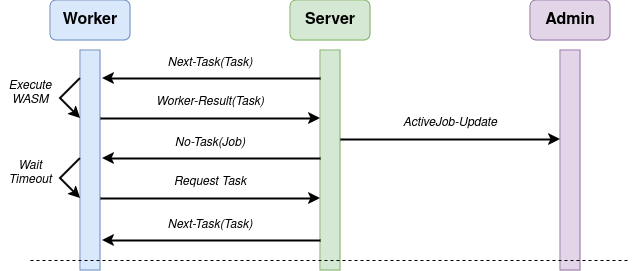
\includegraphics[width=0.95\textwidth]{gfx/figures/communication-timeout.png}
    \caption{Communication: Rescheduling of Tasks after timeout}
    \label{fig:implementation:communication3}
\end{figure}

Each Job has a timeout attribute for its Tasks. Scheduled Tasks that remain incomplete after their allocated timeout period can be redistributed to a different Worker. This mechanism enables the rescheduling of Tasks, which have been assigned to a malfunctioning Worker or a Worker that has disconnected before completing its assigned Task. Additionally, this approach allows rescheduling of Tasks that have been assigned to slower Workers, known as Stragglers, to more efficient Workers. Hence this mechanism can optimize the overall execution time of a Job.

Figure \ref{fig:implementation:communication3} illustrates the case, if all Tasks of the Batch already have been scheduled, but one or more are not yet completed. When a Worker transmits a completed Task to the Server while the timeout period of all other scheduled Tasks has not expired, the Server responds with the \emph{No-Task} message accompanied by the Job object of the currently active Job. The Worker extracts the status and the timeout value from this Job objects and initiates a waiting period equivalent to the timeout value plus a randomized overhead, if the Jobs status is still \emph{RUNNING}. This additional randomized overhead time prevents simultaneous Task requests, if multiple Workers are waiting for a Task at the same time. After the completion of the waiting period, the Worker transmits a \emph{Request Task} message to the Server. The server responds either with a newly available Task or another \emph{No-Task} message, repeating this sequence until the current Batch is fully processed.

\subsection{Persistence}
\label{subsec:implementation:architecture:persistence}
This section describes the persistent data storage implementation of the platform. The primary adressed objective is to ensure system recovery capabilities in cases of system failures, unexpected system crashes, or scheduled system restarts.

The following data objects have been identified as critical for a system recovery:
\begin{itemize}
    \item Job data
    \item Task input arguments
    \item Task results
    \item User credentials
\end{itemize}
Information regarding Workers, their hardware specifications, and operating systems is intentionally excluded from permanent storage.

The system implements a robust persistence mechanism for Job progression. When a running Job is stoped, the current progress and all Task results are automatically saved, hence actively stoping a running Job initiates the persistence process for this Job's current state. This functionality should be utilized if the platform is scheduled to be restarted or terminated.

Additionaly the system persists Job progress after each Batch completion. This mechanism enables periodic Job backups, as each Batch completion establishes a save point. Consequently, the Batch size determines the Job's fallback tolerance in the event of an unexpected system failure.

It is noteworthy that from a Worker's perspective, tasks cannot be persisted. Since WebAssembly is executed in a save sandbox environment the code has usually no access to local files. In the event of an unexpected crash of the Worker's WebAssembly process or browser, the progress of the affected Task will be lost.

\subsubsection{Database}
The PostgreSQL database is used to store the User credentials aswell as each Job object. Each Job object contains a progress attribute that represents a pointer indexing the last completed Task in the Task sequence. During Job recovery, this progress value determines the starting point for the first Task in the new Batch.

\subsubsection{Data in Files}
The system utilizes text files for persistent storage of Task input arguments and Task results. Each Job's critical information about its Tasks is stored in a separate text file for input arguments and the results. 

The method to generate a Batch reads the Task input arguments text file line by line, where each line represents an input argument. For each line, the system creates a unique Task and adds it to the Batch in sequence.

When the progress of a Job is persisted, the Server writes the results of all completed Tasks within the Batch to the Task results text file. Each result is written in a new line, and the results are stored in sequential order.

Additionally the Server implements a special handling mechanism for Tasks that produce files as results. When a Worker transmits such a completed Task, the Server immediately stores the result file in a result directory corresponding to the running Job. Subsequently, when later a Jobs progress is saved, the Server stores the file path to each result in the corresponding Task results text file instead of the actual result data.

\subsection{Scheduling}
\label{subsec:implementation:architecture:scheduling}
The Server is responsible for distributing Tasks from the current Batch to participating Workers. To maximize performance, the Server keeps track of scheduled Tasks to prevent duplicate Task distribution among Workers. The scheduling of Tasks follows the \ac{FIFO} methodology, scheduling the Tasks in sequential order. As described in Section \ref{subsec:implementation:architecture:communication}, each Job entity has a timeout attribute for its Tasks. Only if a Task remains incomplete after its designated timeout period has expired can this Task be rescheduled. This mechanism serves to mitigate issues arising from malfunctioning, disconnected, or straggling Workers.

The scheduling mechanism could be enhanced through the implementation of performance-aware distribution, allocating computationally intensive Tasks to Workers identified as having superior hardware.

\section{Backend}
\label{sec:implementation:backend}
API endpoints 

\section{Frontend}
\label{sec:implementation:frontend}
Design and UI / Pages

\section{Security through Authentication}
\label{sec:implementation:authentication}
How can meliccious use can be prevented?

what is a JWT ? How is JWT used in this project? User vs Admin JWT

\section{Benchmark}
\label{sec:implementation:benchamrk}
Input arguments PNG value transmission etc.

\section{Challenges}
\label{sec:implementation:challenges}
what was difficult?
\begin{itemize}
    \item Hadel Input and Output
    \item Output as File (PNG)
    \item Prevent dublicate Task execution
    \item Minimize Communication
    \item Continue Stoped Job
    \item Implement system recovery
    \item load gluecode and wasm from third party in Webworker
\end{itemize}